\chapter{Ecuaciones de \emph{Hamilton}}

	
\begin{tikzpicture}
	\fill [left color=red!50, right color=teal!50] (0,0) rectangle (6.5,.1);
	\fill [left color=teal!50, right color=blue!50] (6.5,0) rectangle (11.5,.1);
	\end{tikzpicture}

\vspace{1cm}

\begin{adjustwidth}{50pt}{50pt}
\begin{ejemplo}
La formulación hamiltoniana nos dará las ecuaciones de la dinámica. Veremos qué son los momentos generalizados y hablaremos de los teoremas de conservación.
\end{ejemplo}
\end{adjustwidth}
	

\vspace{1cm}
\begin{myblock}{Hamiltoniano y transformada de Legendre. $\ \ H(t)$}

\begin{large}
\begin{equation}
\label{T13inicio}
\boldsymbol{
H(q_i,\ \dot q_i,\ t) \ = \ \sum_{i=1}^n\ \pdv{L}{\dot q_i} \ \dot q_i \ - \ L \, ;
\quad
p_i\ = \ \pdv{L}{\dot q_i} \, ; 
\quad
- \pdv{L}{t} \ = \ \dv{H}{t} }	
\end{equation}
\end{large}
\end{myblock}

\vspace{0.5cm}

\section{Ecuaciones de \emph{Hamilton}}

Sabemos que $\quad \displaystyle f(x,y) \ \to \ \dd f=\pdv{f}{x} \dd x + \pdv{f}{y} \dd y \, ; \quad \text{ si } \ \dd f=xy^2 \dd x + (x+4)\dd y \ \to \ \begin{cases} \ \displaystyle xy^2=\pdv{f}{x} \\ \ \displaystyle x+4=\pdv{f}{y} \end{cases}$
 
Calculemos la diferencial del hamiltoniano, $\boldsymbol{ \ H(q_i,\ \dot q_i,\ t) : \quad\displaystyle \dd H=\sum_{i=1}^n \left[ \pdv{H}{q_i} \dd q_i + \pdv{H}{\dot q_i} \dd \dot q_i \right] + \pdv{H}{t} \dd t } \ (*)$


Como resulta que (ecs. \ref{T13inicio}) $\  \ \displaystyle H=\sum_{i=1}^n \pdv{L}{\dot q_i} \dot q_i - L = \sum_{i=1}^n p_i \dot q_i-L(q_i,\dot q_i,t)\, , \ $ llevado a $\dd H$,


$\displaystyle \dd H = \sum_{i=1}^n \left[
\pdv{p_i \dot q_i}{p_i} \dd p_i + \pdv{p_i \dot q_i}{\dot q_i} \dd \dot q_i
\right] - \dd L =
\sum_{i=1}^n \qty\Big[\dot q_i \dd p_i + p_i \dd \dot q_i] - \dd L$


Incorporemos el diferencial de $L(q_i,\dot q_i,t): \quad \displaystyle \dd L=
\sum_{i=1}^n \left[ \pdv{L}{q_i}\dd q_i + \pdv{L}{\dot q_i} \dd \dot q_i \right] + \pdv{L}{t} \dd t\, , \ $ con lo que

$\displaystyle \dd H = 
\sum_{i=1}^n \qty\Big[\dot q_i \dd p_i + p_i \dd \dot q_i] 
-
\left \{
\sum_{i=1}^n \left[ \pdv{L}{q_i}\dd q_i + \pdv{L}{\dot q_i} \dd \dot q_i \right] + \pdv{L}{t} \dd t
\right\} $

$\displaystyle \dd H = 
\left[
\dot q_i \dd p_i + p_i \dd \dot q_i-\pdv{L}{q_i}\dd q_i -\pdv{L}{\dot q_i} \dd \dot q_i 
\right]
-\pdv{L}{t} \dd t
$

Por las ecuaciones \ref{T13inicio} y las de Euler-Lagrange,

$\displaystyle \dv{t} \left( \pdv{L}{\dot q_i} \right) =\pdv{L}{q_i} \ \to \ \dot p_i=\pdv{L}{q_i}\, ; \quad $  por la trans. Legendre.  $\ \displaystyle \ \dv{t}(p_i)=\dot p_i\, ; \qquad  \ \ \pdv{L}{q_i}=\dot p_i \, ; \ \ \pdv{L}{\dot q_i}=p_i$

Eliminando las cancelaciones, $\boldsymbol{ \qquad \displaystyle \dd H = 
\sum_{i=1}^n \qty\Big[ \ \ \dot q_i \ \dd p_i \ - \ \dot p_i \ \dd  q_i \ ] 
\ - \ \pdv{L}{t} } \ (**)$

Tenemos el diferencial del hamiltoniano expresado de dos forma distintas, genéricamente, a partir de las variables de que depende $(*)$ y a partir de su definición explícita y de las ecuaciones de Euler-Lagrange (que son el ingrediente necesario para conocer la dinámica de la partícula, equivalentes a las ecuaciones de Newton) $(**)$.

$\begin{cases}
\ (*) \ \ \ \boldsymbol{\displaystyle \dd H=\sum_{i=1}^n \left[ \textcolor{red}{\pdv{H}{q_i} \dd q_i} +  \textcolor{blue}{\pdv{H}{\dot q_i} \dd \dot q_i} \right] + \pdv{H}{t} \dd t } 
\\ \\
\ (**)\ \ \boldsymbol{\displaystyle \dd H = 
\sum_{i=1}^n \qty\Big[ \ \  \textcolor{blue}{\dot q_i \ \dd p_i} \  \textcolor{red}{- \ \dot p_i \ \dd  q_i} \ ] 
\ - \ \pdv{L}{t} \dd t } 
\end{cases} \ \ $  Comparando ambas expresiones,

\vspace{5mm}
\begin{myalertblock}{Ecuaciones de Hamilton}
\vspace{3mm}
\begin{large}
\begin{equation}
\label{T13eccHamilton}
\boldsymbol{
\boxed{ \ 
\dot q_i = \pdv{H}{p_i} 
\ }
\qquad \quad 
\boxed{ \
\dot p_i=-\pdv{H}{q_j}
\ }
\qquad \quad \text{además} \quad
-\pdv{L}{t}=\pdv{H}{t}
}	
\end{equation}	
\end{large}	
\end{myalertblock}

\vspace{5mm}
En el capítulo anterior vimos que

\begin{equation}
\tag{\ref{T9Hdet}}
 \boldsymbol{	-\pdv{L}{t} \ = \ \dv{H}{t} } 
\end{equation}

\underline{conclusión}:

\begin{large}
\begin{equation}
\label{T13HdeT}
\subrayado{\boxed{ \  \boldsymbol{	 \dv{H}{t}\  = \ \pdv{H}{t}  }  \ }}
\end{equation}
\end{large}

Para ver si $\displaystyle \dv{H}{t}$ cambia con $t$ basta con calcular $\ \displaystyle \pdv{H}{t}\, , \  $ comprobar si $t$ aparece explícitamente en el hamiltoniano $H$, si no es así, $\displaystyle \pdv{H}{t}=0=\dv{H}{t} \ \to \ H \ $ constante de movimiento.

\vspace{5mm}

\begin{myalertblock}{$H$ constante del movimiento}
\begin{large}
\begin{equation}
\label{T13HdeT2}
	\boldsymbol{ H \ \neq \ H(t ) \quad \Rightarrow \quad H \ \text{constante del movimiento} }
\end{equation}	
\end{large}
\end{myalertblock}

\vspace{10mm}

\begin{ejemplo}
\vspace{2mm}
\underline{Reflexión}:

--- ?`Qué es mejor usar $L$ o $H$ para resolver problemas?

--- Sin duda, $L$, el lagrangiano, es más sencillo para resolver las ecuaciones de movimiento.

--- ?`Y para que vemos $H$?

--- $H$ es muy potente y si se desea profundizar en la estructura de la mecánica (leyes de conservación y simetrías) y extenderlos a mecánica cuántica o teoría cuántica de campos en imprescindible conocerlo (históricamente empezaron así las teorías cuánticas).
\vspace{2mm}
\end{ejemplo}

\vspace{10mm}

\subsection{Ejemplo de las ecuaciones de \emph{Hamilton}}
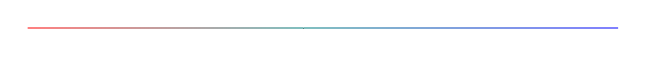
\begin{tikzpicture}
	\fill [left color=red!50, right color=teal!50] (0,0) rectangle (3.5,.01);
	\fill [left color=teal!50, right color=blue!50] (3.5,0) rectangle (7.5,.01);
	\end{tikzpicture}
\vspace{0.5cm}


\begin{example}
	
	\begin{multicols}{2}
	\begin{figure}[H]
	\centering
	\includegraphics[width=.4\textwidth]{imagenes/img13-01.png}
\end{figure}


\vspace{2mm} El palo  está obligado (motor externo) a oscilar con velocidad angular constate $ \ \theta=\omega\ t$

\vspace{2mm} La masa $m$ se puede mover libremente, sin fricción,  por el palo. 

\vspace{2mm} ?`Cuál será el movimiento de $m$ sometida a esta restricción?

\end{multicols}
\end{example}
\vspace{5mm}

$\begin{cases}
\ x=r\cos \theta = r \cos (\omega t)	 \\ \  y=r\sin \theta = r \sin (\omega t)
\end{cases} \qquad 
\begin{cases}
\ \dot x= \dot r \cos \omega t - \omega r \sin \omega t \\ 	
\ \dot y= \dot r \sin \omega t + \omega r \cos \omega t
\end{cases}$

$T=\dfrac m 2 \left(
( \dot r \cos \omega t - \omega r \sin \omega t )^2 + 	
(  \dot r \sin \omega t + \omega r \cos \omega t )^2
\right) = $

$\displaystyle T=
\dfrac m 2 ( \dot r^2 \cos^2 \omega t +r^2\omega^2 \sin^2 \omega t - \cancel{2r \ \dot r \ \omega \sin (\omega t) \cos (\omega t)} +
\dot r^2 \sin^2 \omega t +r^2\omega^2 \cos^2 \omega t + \cancel{2r \ \dot r  \ \omega \sin (\omega t) \cos (\omega t))}$

$T= \dfrac m 2 (\dot r^2 + r^2 \omega^2)$

$\boldsymbol{ L }= \dfrac m 2 (\dot r^2 + r^2 \omega^2) - mgy = \boldsymbol{\dfrac m 2 \ (\dot r^2 + r^2 \omega^2)\  - \ mg \ r\sin \omega t }$

Vamos a por el hamiltoniano $H$. Nuestra única coordenada generalizada es $\ r$:

$p_r=\displaystyle \pdv{L}{\dot r} = \dfrac m 2 \ 2 \dot r =m\dot r \ \to \ \dot r=\dfrac {p_r} m \ 	\ \ \textcolor{gris}{ (3*)}$

$H=\displaystyle \pdv{L}{\dot r} \dot r - L = p_r \dot r - L = p_r \dfrac m 2 - [\dot r^2 + \dfrac m 2 r^2 \omega ^2 - mg\ r \sin \omega t ]  $

$ \textcolor{gris}{ (3*)} \ \to \ H = \displaystyle p_r \dfrac{p_r}{m} - \dfrac m 2 \left( \dfrac{p_r}{m} \right)^2 - \dfrac m 2 r^2 \omega^2 +mr \ r \sin \omega t$

\begin{equation}
\label{T13Hejemplo}	
\boldsymbol{ H \ = \ \dfrac{p_r^2}{m} \ - \ \dfrac m 2 r^2 \omega^2 \ + \ mg\ r \sin \omega t } \ \ \ \textcolor{gris}{  \neq \ E }
\end{equation}

\begin{small} \textcolor{gris}{$ H \neq \ E \ $  pues $\ H \neq T+V \ $ ya que  $\dfrac{p_r^2}{m}  -  \dfrac m 2 r^2 \omega^2 \neq T$} \end{small}

\vspace{5mm} Vamos, ahora, a por las ecuaciones de Hamilton (ecuaciones del movimiento):

$\textcolor{gris}{\dot q_j=\displaystyle \pdv {H}{p_j}} \ \to \    \boldsymbol{\dot r = } \displaystyle \pdv{H}{p} \boldsymbol{ = \dfrac p m}\qquad \qquad  \textcolor{gris}{ \dot p_j= - \displaystyle \pdv {H}{q_j} } \ \to \    \boldsymbol{\dot p = } - \displaystyle \pdv{H}{r} \boldsymbol{ = mr^2\omega^2 -mg \sin \omega t}$

\begin{large}
\begin{equation}
\label{T13EcMovto-ejemplo}	
\boldsymbol{
\subrayado{\dot r =  \dfrac p m}
\qquad \qquad \qquad
\subrayado{\dot p  = mr^2\omega^2 -mg \sin \omega t}
}
\end{equation}
\end{large}

Una estrategia para la solución es , despejando de la primera de las ecuaciones de movimiento (ec \ref{T13EcMovto-ejemplo}) $ \ \dot r =  \dfrac p m \, , \ $ derivando, $ \ \ddot r =  \dfrac {\dot p} {m} \ \to \ \dot p = m \ddot r \ $ y sustituyendo en la segunda ecuación,

\begin{equation}
\boldsymbol{m \ \ddot r \ = \ m \ r \ \omega^2 \ - \ m\ g\ r \sin \omega t}
\end{equation}

Obtenemos una sola EDO que se puede resolver, por ejemplo, numéricamente con el sw. adecuado.

\vspace{1cm}
\section{Leyes de conservación}
\vspace{0.5cm}

\begin{definition}

\begin{myblock}{Momento canónico generalizado}
\begin{large}
\begin{equation}
\label{T13MomentoCanonicoGeneralizado}	
\text{Se llama } \textbf{ \emph{momento canónico generalizado} } \qquad  \boldsymbol{ p_i \ = \ \pdv{L}{\dot q_i} }
\end{equation}
\end{large}
\end{myblock}	
\end{definition}

\vspace{5mm}
Bajo las siguientes dos premisas,

\begin{enumerate}[a) ]
\item $\boldsymbol T$ es función homogénea de grado 2.
\item $\boldsymbol V$ solo depende de las coordenadas generalizadas $q_j$	
\end{enumerate}

se cumple (en este contexto):

\begin{itemize}
\item si $\boldsymbol{ H \neq H(q) } \quad \to \quad \dot p_j =\textcolor{gris}{-\displaystyle \pdv{H}{q_j}} = 0 \quad \to \quad \boxed{ \boldsymbol {p_i} \textbf{ es cte. del movimiento.}}$	
\item si $\boldsymbol{ H \neq H(t) } \quad \to \quad \displaystyle \dv{H}{t} =\textcolor{gris}{\pdv{H}{t}} = 0 \quad \to \quad \boxed{ \boldsymbol {H} \textbf{ es cte. en el tiempo.}}$	
\end{itemize}

\vspace{10mm}

Pensemos que deseamos construir una \emph{nueva teoría} con las siguientes peticiones:

\begin{enumerate}[I ]
\item  Deseamos que nuestra teoría sea valida ahora, en el pasado y esperamos que también lo sea en el futuro.
\item  Deseamos que las leyes de nuestra teoría no dependan de donde se encuentra nuestro observador (\emph{homogeneidad}).
\item Y que tampoco dependan de su orientación (\emph{isotropía}).
\end{enumerate}

Es decir, que las leyes que obtengamos con nuestra nueva teoría sean \emph{\textbf{invariantes} en el tiempo, ante traslaciones y ante rotaciones.}

\textcolor{gris}{La teoría de la relatividad especial de Einstein se basa en estas tres peticiones y, ademas, en IV) que la velocidad de la luz , $c$, sea constante y que V) las leyes sean invariantes ante cualquier cambio de sistema de referencia inercial}.

Los postulados I), II) y III) son básicos para cualquier teoría física y según se vayan añadiendo más postulados se obtienen una teorías u otras.

Además, nuestras teorías, en los límites adecuados, deben reproducir lo que ya conocemos y funciona.

Las leyes de conservación (y las simetrías, teorema de Noether que veremos en el próximo capítulo) son conceptos muy profundos que nos ayudan, no solo a entender nuestras teorías, sino a la hora de explicar nuevas teorías. Veremos (próximo tema) que para cada ley de conservación existe una simetría asociada.



\vspace{10mm}


\subsection{Ejemplo de los teoremas de conservación}
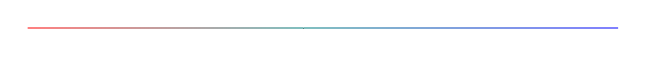
\begin{tikzpicture}
	\fill [left color=red!50, right color=teal!50] (0,0) rectangle (3.5,.01);
	\fill [left color=teal!50, right color=blue!50] (3.5,0) rectangle (7.5,.01);
	\end{tikzpicture}
\vspace{0.5cm}


\begin{example}

	\begin{figure}[H]
	\centering
	\includegraphics[width=.95\textwidth]{imagenes/img13-03.png}
\end{figure}

\begin{center}$m$ sobre la mesa (no influye $g$), sin fricción, unida al muelle $k$\end{center}
\end{example}
\vspace{5mm}

En la sección \ref{T12Tesfericas} vimos la expresión de la energía cinética en coordenadas esféricas,

$T \ = \ \dfrac m 2 \ (\ \ \dot r^2 \ + \ r^2 \ \dot \theta^2 \ + \ r^2 \ \sin^2 \theta \ \dot \phi^2 \ ) \  $ En nuestro caso, $\theta=\pi/2;\ \dot \theta=0 \, , \ $ tenemos:

$T=\dfrac m 2 (\dot r^2+r^2 \dot \phi^2) \ $  

La energía potencial es, $\ V=\dfrac k 2 \left( \sqrt{x^2+y^2} - a \right)^2=\dfrac k 2 (r-a)^2$; $\ \ a=$ longitud natural del muelle.

El langrangiano:  $\ \ \ \boldsymbol { L= \dfrac m 2 (\dot r^2+r^2 \dot \phi^2)  - \dfrac k 2 (r-a)^2 }$

Como $T$ es homogénea de grado 2 \textcolor{gris}{$(T(\lambda \dot r, \lambda \dot \phi)=\lambda^2 T(\dot r, \dot \phi))$}  y $V=V(r)$ \textcolor{gris}{(pero $V \neq V(\dot r)$)}, entonces, $\ \boldsymbol{H=E.\ }$  Como $\ E=T+V\, , \ $ tenemos un modo sencillo de calcular el hamiltoniano:

$$\boldsymbol {H}=E=T+V=\boldsymbol { \dfrac m 2 (\dot r^2+r^2 \dot \phi^2)  \ + \  \dfrac k 2 (r-a)^2 }$$

Para las ecuaciones de Hamilton, necesitamos  calcular $p_r$ y $p_\phi$:

$p_r=\displaystyle \pdv{H}{\dot r}=m\dot r \ \to \ \dot r=\dfrac{p_r}{m}\, ; \qquad \qquad
p_\phi=\displaystyle \pdv{H}{\dot \phi}=m r^2 \dot \phi \ \to \ \dot \phi=\dfrac{p_\phi}{mr^2}$

Sustituyendo en el hamiltoniano:

$H=\dfrac m 2 \left( \dfrac{p_r}{m} \right)^2 + \dfrac m 2 r^2 \left( \dfrac{p_\phi}{mr^2} \right)^2+\dfrac k 2 (r-a)^2 = \dfrac{p_r^2}{2m} + \dfrac{p_\phi^2}{2mr^2} + \dfrac k 2 (r-a)^2$

\vspace{5mm} \textbf{?`Qué se conserva aquí?}

$q_1=r\, ; \ q_r=\phi \ $ y vemos que $  H=H(r)	 \ $ pero $\ H \neq H(\phi) \ $, por lo que podemos asegurar que $ \ \dot p_\phi=0 \ \to \ p_\phi=$ constante del movimiento. Tradicionalmente se le llama, $\ mr^2 \dot \phi=L_z=cte$

Como $H$ no depende explícitamente de $t,\ \ H\neq H(t)\  \to \ H=E\, , \ $ la energía se conserva, es constante en el tiempo:

$\boldsymbol{ \displaystyle
\dfrac{m^2 \dot r^2}{2m} \ + \ \dfrac{L_z^2}{2mr^2} \ + \ \dfrac{k(r-a)^2}{2} \ = \ E \ = \ cte
}
\qquad \qquad \qquad 
p_r=m\dot r\, ; \quad p_\phi=mr^2 \dot \phi$

\vspace{5mm} Si despejamos $\dot r  \to \ \dot r=\sqrt{
\dfrac 2 m \ \left[
E-\dfrac{L_z^2}{2mr^2}-\dfrac{k(r-a)^2}{2}
\right]}
\displaystyle = \dv{r}{t}\, , \  $ separando e integrando,


$\sqrt{\dfrac m 2 } \ \displaystyle \int \dfrac{1}{\sqrt{E-\dfrac{L_z^2}{2mr^2}-\dfrac{k(r-a)^2}{2}}} \ \dd r \ = \ \int \ \dd t \ = \ t + A(cte)$  
 
Integral que se puede consultar en tablas. El hecho de que $E=cte$ y que $p_\phi=cte$ permiten resolver \emph{formalmente} el problema.


En el siguiente capítulo veremos el importantísimo, en física teórica, teorema de Noether: siempre que hay una ley de conservación es porque hay una simetría continua.



